\documentclass[12pt,a4paper,openany]{book}

\usepackage{lmodern}
\usepackage[svgnames]{xcolor} % Required to specify font color
\usepackage{xcolor}
\definecolor{vert1}{rgb}{0.0,0.3.9,0.0}
\definecolor{bleu}{rgb}{0,0,0.5}
\definecolor{bleu3}{rgb}{1,0.2,0.2}
\definecolor{grisgris}{gray}{0.4}
\definecolor{grisclair}{HTML}{E7E7E7}
\definecolor{grisfonce}{HTML}{A5A5A5}
\definecolor{rougeUPS}{rgb}{0.6, 0.3, 0.3}

\fboxsep =0pt \parindent =0pt\parskip =12pt



\usepackage[utf8]{inputenc}
\usepackage[T1]{fontenc}
\usepackage[francais]{babel}
\usepackage[top=1.7cm, bottom=1.7cm, left=1.7cm, right=1.7cm]{geometry}
\usepackage{verbatim}
\usepackage[urlbordercolor={1 1 1}, linkbordercolor={1 1 1}, linkcolor=vert1, urlcolor=bleu, colorlinks=true]{hyperref}
\usepackage{tikz} %Vectoriel
\usepackage{listings}
\usepackage{fancyhdr}
\usepackage{multido}
\usepackage{amssymb}
\usepackage{graphicx} % Required for box manipulation
\usepackage{float}

\newcommand{\titre}{Traduction de langages}
\newcommand{\subtitle}{TL}
\newcommand{\auteur}{Antoine de \bsc{Roquemaurel}}
\newcommand{\formation}{M1 Informatique -- Développement Logiciel}
\newcommand{\semestre}{7}
\newcommand{\annee}{2014}
\newcommand{\prof}{Christine \bsc{Maurel}}


\newcommand{\pole}{}
\newcommand{\sigle}{oim}
\newcommand{\logo}{/home/aroquemaurel/cours/templates/templates/ups.jpg}
\definecolor{gris1}{gray}{0.40}
\definecolor{gris2}{gray}{0.55}
\definecolor{gris3}{gray}{0.65}
\definecolor{gris4}{gray}{0.50}
\definecolor{vert}{rgb}{0,0.4,0}
\definecolor{violet}{rgb}{0.65, 0.2, 0.65}
\definecolor{bleu1}{rgb}{0,0,0.8}
\definecolor{bleu2}{rgb}{0,0.2,0.6}
\definecolor{bleu3}{rgb}{0,0.2,0.2}
\definecolor{rouge}{HTML}{F93928}


\lstdefinelanguage{algo}{%
   morekeywords={%
    %%% couleur 1
		importer, programme, glossaire, fonction, procedure, constante, type, 
	%%% IMPORT & Co.
		si, sinon, alors, fin, tantque, debut, faire, lorsque, fin lorsque, 
		declenche, declencher, enregistrement, tableau, retourne, retourner, =, pour, a,
		/=, <, >, traite,exception, 
	%%% types 
		Entier, Reel, Booleen, Caractere, Réél, Booléen, Caractère,
	%%% types 
		entree, maj, sortie,entrée,
	%%% types 
		et, ou, non,
	},
  sensitive=true,
  morecomment=[l]{--},
  morestring=[b]',
}

\lstset{language=algo,
    %%% BOUCLE, TEST & Co.
      emph={importer, programme, glossaire, fonction, procedure, constante, type},
      emphstyle=\color{bleu2},
    %%% IMPORT & Co.  
	emph={[2]
		si, sinon, alors, fin , tantque, debut, faire, lorsque, fin lorsque, 
		declencher, retourner, et, ou, non,enregistrement, retourner, retourne, 
		tableau, /=, <, =, >, traite,exception, pour, a
	},
      emphstyle=[2]\color{bleu1},
    %%% FONCTIONS NUMERIQUES
      emph={[3]Entier, Reel, Booleen, Caractere, Booléen, Réél, Caractère},
      emphstyle=[3]\color{gris1},
    %%% FONCTIONS NUMERIQUES
      emph={[4]entree, maj, sortie, entrée},	
      emphstyle=[4]\color{gris1},
}
\lstdefinelanguage{wl}{%
   morekeywords={%
    %%% couleur 1
		importer, programme, glossaire, fonction, procedure, constante, type, 
	%%% IMPORT & Co.
		si, sinon, alors, fin, TANTQUE, tantque, FIN, PROCEDURE, debut, faire, lorsque, 
		fin lorsque, declenche, declencher, enregistrement, tableau, retourne, retourner, =, 
		/=, <, >, traite,exception, 
	%%% types 
		Entier, Reel, Booleen, Caractere, Réél, Booléen, Caractère,
	%%% types 
		entree, maj, sortie,entrée,
	%%% types 
		et, ou, non,
	},
  sensitive=true,
  morecomment=[l]{//},
  morestring=[b]',
}

\lstset{language=wl,
    %%% BOUCLE, TEST & Co.
      emph={importer, programme, glossaire, fonction, procedure, constante, type},
      emphstyle=\color{bleu2},
    %%% IMPORT & Co.  
	emph={[2]
		si, sinon, alors, fin , tantque, debut, faire, lorsque, fin lorsque, 
		declencher, retourner, et, ou, non,enregistrement, retourner, retourne, 
		tableau, /=, <, =, >, traite,exception
	},
      emphstyle=[2]\color{bleu1},
    %%% FONCTIONS NUMERIQUES
      emph={[3]Entier, Reel, Booleen, Caractere, Booléen, Réél, Caractère},
      emphstyle=[3]\color{gris1},
    %%% FONCTIONS NUMERIQUES
      emph={[4]entree, maj, sortie, entrée},	
      emphstyle=[4]\color{gris1},
}
\lstdefinelanguage{css}{%
   morekeywords={%
    %%% couleur 1
		background, image, repeat, position, index, color, border, font, 
		size, url, family, style, variant, weight, letter, spacing, line, 
		height, text, decoration, align, indent, transform, shadow, 
		background, image, repeat, position, index, color, border, font, 
		size, url, family, style, variant, weight, letter, spacing, line, 
		height, text, decoration, align, indent, transform, shadow, 
		vertical, align, white, space, word, spacing,attachment, width, 
		max, min, margin, padding, clip, direction, display, overflow,
		visibility, clear, float, top, right, bottom, left, list, type, 
		collapse, side, empty, cells, table, layout, cursor, marks, page, break,
		before, after, inside, orphans, windows, azimuth, after, before, cue, 
		elevation, pause, play, during, pitch, range, richness, spek, header, 
		numeral, punctuation, rate, stress, voice, volume,
	%%% types 
		left, right, bottom, top, none, center, solid, black, blue, red, green,
	},
  sensitive=true,
  sensitive=true,
  morecomment=[s]{/*}{*/},
  morestring=[b]',
}
\lstset{language=css,
    %%% BOUCLE, TEST & Co.
      emph={
		background, image, repeat, position, index, color, border, font, 
		size, url, family, style, variant, weight, letter, spacing, line, 
		height, text, decoration, align, indent, transform, shadow, 
		background, image, repeat, position, index, color, border, font, 
		size, url, family, style, variant, weight, letter, spacing, line, 
		height, text, decoration, align, indent, transform, shadow, 
		vertical, align, white, space, word, spacing,attachment, width, 
		max, min, margin, padding, clip, direction, display, overflow,
		visibility, clear, float, top, right, bottom, left, list, type, 
		collapse, side, empty, cells, table, layout, cursor, marks, page, break,
		before, after, inside, orphans, windows, azimuth, after, before, cue, 
		elevation, pause, play, during, pitch, range, richness, spek, header, 
		numeral, punctuation, rate, stress, voice, volume,
	  },
      emphstyle=\color{bleu2},
    %%% FONCTIONS NUMERIQUES
      emph={[3]
		left, right, bottom, top,none, solid, black, blue, green,
		  },
      emphstyle=[3]\color{bleu3},
    %%% FONCTIONS NUMERIQUES
}

\lstset{language=SQL,
    %%% BOUCLE, TEST & Co.
      emph={INSERT, UPDATE, DELETE, WHERE, SET, GROUP, BY, ORDER, REFERENCES},
      emphstyle=\color{bleu2},
    %%% IMPORT & Co.  
	emph={[2]
		if, end, begin, then, for, each, else, after, of, on, to
	},
      emphstyle=[2]\color{bleu1},
    %%% FONCTIONS NUMERIQUES
      emph={[3]Entier, Reel, Booleen, Caractere, Booléen, Réél, Caractère},
      emphstyle=[3]\color{gris1},
    %%% FONCTIONS NUMERIQUES
      emph={[4]entree, maj, sortie, entrée},	
      emphstyle=[4]\color{gris1},
}
\lstdefinelanguage{ARM}{%
   morekeywords={%
   ADD, SUB, MOV, MUL, RSB,CMP, BLS, BLE, B,BHI,LDR,
   BGE, RSBLT, BGT, BEQ, BNE,BLT,BHS,STR,STRB
	},
  sensitive=true,
  morecomment=[l]{@},
  morestring=[b]',
}

\lstset{ % general style for listings 
   numbers=left 
   , literate={é}{{\'e}}1 {è}{{\`e}}1 {à}{{\`a}}1 {ê}{{\^e}}1 {É}{{\'E}}1 {ô}{{\^o}}1 {€}{{\euro}}1{°}{{$^{\circ}$}}1 {ç}{ {c}}1 {ù}{u}1
	, extendedchars=\true
   , tabsize=2 
   , frame=l
   , framerule=1.1pt
   , linewidth=520px
   , breaklines=true 
   , basicstyle=\footnotesize\ttfamily 
   , numberstyle=\tiny\ttfamily 
   , framexleftmargin=0mm 
   , xleftmargin=0mm 
   , captionpos=b 
	, keywordstyle=\color{bleu2}
	, commentstyle=\color{vert}
	, stringstyle=\color{rouge}
	, showstringspaces=false
	, extendedchars=true
	, mathescape=true
} 
%	\lstlistoflistings
%	\addcontentsline{toc}{part}{List of code examples}
 %prise en charge du langage algo
\documentclass[12pt,a4paper,openany]{book}
\usepackage{lmodern}
\usepackage{xcolor}
\usepackage{xcolor}
\definecolor{vert1}{rgb}{0.0,0.3.9,0.0}
\definecolor{bleu}{rgb}{0,0,0.5}
\definecolor{bleu3}{rgb}{1,0.2,0.2}
\definecolor{grisgris}{gray}{0.4}
\definecolor{grisclair}{HTML}{E7E7E7}
\definecolor{grisfonce}{HTML}{A5A5A5}
\definecolor{rougeUPS}{rgb}{0.6, 0.3, 0.3}

\fboxsep =0pt \parindent =0pt\parskip =12pt



\usepackage[utf8]{inputenc}
\usepackage[T1]{fontenc}
\usepackage[francais]{babel}
\usepackage[top=1.7cm, bottom=1.7cm, left=1.7cm, right=1.7cm]{geometry}
\usepackage{verbatim}
\usepackage[urlbordercolor={1 1 1}, linkbordercolor={1 1 1}, linkcolor=vert1, urlcolor=bleu, colorlinks=true]{hyperref}
\usepackage{tikz} %Vectoriel
\usepackage{listings}
\usepackage{fancyhdr}
\usepackage{multido}
\usepackage{amssymb}
\usepackage{float}

\newcommand{\titre}{Complexité des algorithmes}

\newcommand{\pole}{}
\newcommand{\sigle}{complexite}

\newcommand{\semestre}{3}

\definecolor{gris1}{gray}{0.40}
\definecolor{gris2}{gray}{0.55}
\definecolor{gris3}{gray}{0.65}
\definecolor{gris4}{gray}{0.50}
\definecolor{vert}{rgb}{0,0.4,0}
\definecolor{violet}{rgb}{0.65, 0.2, 0.65}
\definecolor{bleu1}{rgb}{0,0,0.8}
\definecolor{bleu2}{rgb}{0,0.2,0.6}
\definecolor{bleu3}{rgb}{0,0.2,0.2}
\definecolor{rouge}{HTML}{F93928}


\lstdefinelanguage{algo}{%
   morekeywords={%
    %%% couleur 1
		importer, programme, glossaire, fonction, procedure, constante, type, 
	%%% IMPORT & Co.
		si, sinon, alors, fin, tantque, debut, faire, lorsque, fin lorsque, 
		declenche, declencher, enregistrement, tableau, retourne, retourner, =, pour, a,
		/=, <, >, traite,exception, 
	%%% types 
		Entier, Reel, Booleen, Caractere, Réél, Booléen, Caractère,
	%%% types 
		entree, maj, sortie,entrée,
	%%% types 
		et, ou, non,
	},
  sensitive=true,
  morecomment=[l]{--},
  morestring=[b]',
}

\lstset{language=algo,
    %%% BOUCLE, TEST & Co.
      emph={importer, programme, glossaire, fonction, procedure, constante, type},
      emphstyle=\color{bleu2},
    %%% IMPORT & Co.  
	emph={[2]
		si, sinon, alors, fin , tantque, debut, faire, lorsque, fin lorsque, 
		declencher, retourner, et, ou, non,enregistrement, retourner, retourne, 
		tableau, /=, <, =, >, traite,exception, pour, a
	},
      emphstyle=[2]\color{bleu1},
    %%% FONCTIONS NUMERIQUES
      emph={[3]Entier, Reel, Booleen, Caractere, Booléen, Réél, Caractère},
      emphstyle=[3]\color{gris1},
    %%% FONCTIONS NUMERIQUES
      emph={[4]entree, maj, sortie, entrée},	
      emphstyle=[4]\color{gris1},
}
\lstdefinelanguage{wl}{%
   morekeywords={%
    %%% couleur 1
		importer, programme, glossaire, fonction, procedure, constante, type, 
	%%% IMPORT & Co.
		si, sinon, alors, fin, TANTQUE, tantque, FIN, PROCEDURE, debut, faire, lorsque, 
		fin lorsque, declenche, declencher, enregistrement, tableau, retourne, retourner, =, 
		/=, <, >, traite,exception, 
	%%% types 
		Entier, Reel, Booleen, Caractere, Réél, Booléen, Caractère,
	%%% types 
		entree, maj, sortie,entrée,
	%%% types 
		et, ou, non,
	},
  sensitive=true,
  morecomment=[l]{//},
  morestring=[b]',
}

\lstset{language=wl,
    %%% BOUCLE, TEST & Co.
      emph={importer, programme, glossaire, fonction, procedure, constante, type},
      emphstyle=\color{bleu2},
    %%% IMPORT & Co.  
	emph={[2]
		si, sinon, alors, fin , tantque, debut, faire, lorsque, fin lorsque, 
		declencher, retourner, et, ou, non,enregistrement, retourner, retourne, 
		tableau, /=, <, =, >, traite,exception
	},
      emphstyle=[2]\color{bleu1},
    %%% FONCTIONS NUMERIQUES
      emph={[3]Entier, Reel, Booleen, Caractere, Booléen, Réél, Caractère},
      emphstyle=[3]\color{gris1},
    %%% FONCTIONS NUMERIQUES
      emph={[4]entree, maj, sortie, entrée},	
      emphstyle=[4]\color{gris1},
}
\lstdefinelanguage{css}{%
   morekeywords={%
    %%% couleur 1
		background, image, repeat, position, index, color, border, font, 
		size, url, family, style, variant, weight, letter, spacing, line, 
		height, text, decoration, align, indent, transform, shadow, 
		background, image, repeat, position, index, color, border, font, 
		size, url, family, style, variant, weight, letter, spacing, line, 
		height, text, decoration, align, indent, transform, shadow, 
		vertical, align, white, space, word, spacing,attachment, width, 
		max, min, margin, padding, clip, direction, display, overflow,
		visibility, clear, float, top, right, bottom, left, list, type, 
		collapse, side, empty, cells, table, layout, cursor, marks, page, break,
		before, after, inside, orphans, windows, azimuth, after, before, cue, 
		elevation, pause, play, during, pitch, range, richness, spek, header, 
		numeral, punctuation, rate, stress, voice, volume,
	%%% types 
		left, right, bottom, top, none, center, solid, black, blue, red, green,
	},
  sensitive=true,
  sensitive=true,
  morecomment=[s]{/*}{*/},
  morestring=[b]',
}
\lstset{language=css,
    %%% BOUCLE, TEST & Co.
      emph={
		background, image, repeat, position, index, color, border, font, 
		size, url, family, style, variant, weight, letter, spacing, line, 
		height, text, decoration, align, indent, transform, shadow, 
		background, image, repeat, position, index, color, border, font, 
		size, url, family, style, variant, weight, letter, spacing, line, 
		height, text, decoration, align, indent, transform, shadow, 
		vertical, align, white, space, word, spacing,attachment, width, 
		max, min, margin, padding, clip, direction, display, overflow,
		visibility, clear, float, top, right, bottom, left, list, type, 
		collapse, side, empty, cells, table, layout, cursor, marks, page, break,
		before, after, inside, orphans, windows, azimuth, after, before, cue, 
		elevation, pause, play, during, pitch, range, richness, spek, header, 
		numeral, punctuation, rate, stress, voice, volume,
	  },
      emphstyle=\color{bleu2},
    %%% FONCTIONS NUMERIQUES
      emph={[3]
		left, right, bottom, top,none, solid, black, blue, green,
		  },
      emphstyle=[3]\color{bleu3},
    %%% FONCTIONS NUMERIQUES
}

\lstset{language=SQL,
    %%% BOUCLE, TEST & Co.
      emph={INSERT, UPDATE, DELETE, WHERE, SET, GROUP, BY, ORDER, REFERENCES},
      emphstyle=\color{bleu2},
    %%% IMPORT & Co.  
	emph={[2]
		if, end, begin, then, for, each, else, after, of, on, to
	},
      emphstyle=[2]\color{bleu1},
    %%% FONCTIONS NUMERIQUES
      emph={[3]Entier, Reel, Booleen, Caractere, Booléen, Réél, Caractère},
      emphstyle=[3]\color{gris1},
    %%% FONCTIONS NUMERIQUES
      emph={[4]entree, maj, sortie, entrée},	
      emphstyle=[4]\color{gris1},
}
\lstdefinelanguage{ARM}{%
   morekeywords={%
   ADD, SUB, MOV, MUL, RSB,CMP, BLS, BLE, B,BHI,LDR,
   BGE, RSBLT, BGT, BEQ, BNE,BLT,BHS,STR,STRB
	},
  sensitive=true,
  morecomment=[l]{@},
  morestring=[b]',
}

\lstset{ % general style for listings 
   numbers=left 
   , literate={é}{{\'e}}1 {è}{{\`e}}1 {à}{{\`a}}1 {ê}{{\^e}}1 {É}{{\'E}}1 {ô}{{\^o}}1 {€}{{\euro}}1{°}{{$^{\circ}$}}1 {ç}{ {c}}1 {ù}{u}1
	, extendedchars=\true
   , tabsize=2 
   , frame=l
   , framerule=1.1pt
   , linewidth=520px
   , breaklines=true 
   , basicstyle=\footnotesize\ttfamily 
   , numberstyle=\tiny\ttfamily 
   , framexleftmargin=0mm 
   , xleftmargin=0mm 
   , captionpos=b 
	, keywordstyle=\color{bleu2}
	, commentstyle=\color{vert}
	, stringstyle=\color{rouge}
	, showstringspaces=false
	, extendedchars=true
	, mathescape=true
} 
%	\lstlistoflistings
%	\addcontentsline{toc}{part}{List of code examples}
 %prise en charge du langage C 
\date{\today}

\makeindex
\lfoot{Université Toulouse III -- Paul Sabatier}
\rfoot{\sigle\semestre}
%\rfoot{}
\cfoot{}
\makeglossary
\makeatletter
\def\clap#1{\hbox to 0pt{\hss #1\hss}}%
\def\ligne#1{%
\hbox to \hsize{%
\vbox{\centering #1}}}%
\def\haut#1#2#3{%
\hbox to \hsize{%
\rlap{\vtop{\raggedright #1}}%
\hss
\clap{\vtop{\centering #2}}%
\hss
\llap{\vtop{\raggedleft #3}}}}%
\def\bas#1#2#3{%
\hbox to \hsize{%
\rlap{\vbox{\raggedright #1}}%
\hss \clap{\vbox{\centering #2}}%
\hss
\llap{\vbox{\raggedleft #3}}}}%
\def\maketitle{%
\thispagestyle{empty}\vbox to \vsize{%
\haut{}{\@blurb}{}

\vfill
\vspace{1cm}
\begin{flushleft}
\usefont{OT1}{ptm}{m}{n}
\huge \@title
\end{flushleft}
\par
\hrule height 4pt
\par
\begin{flushright}
\usefont{OT1}{phv}{m}{n}
\Large \@author
\par
\end{flushright}
\vspace{1cm}
\vfill
\vfill
\bas{}{\@location, le \@date}{}
}%
\cleardoublepage
}
\def\date#1{\def\@date{#1}}
\def\author#1{\def\@author{#1}}
\def\title#1{\def\@title{#1}}
\def\location#1{\def\@location{#1}}
\def\blurb#1{\def\@blurb{#1}}
\date{\today}
\author{}
\title{}
\location{Amiens}\blurb{}
\makeatother
\title{\titre}
\author{Semestre \semestre}

\location{Toulouse}
\blurb{%
Université Toulouse III -- Paul sabatier\\
L2 Informatique\\
}%



%\title{Cours \\ \titre}
%\date{\today\\ Semestre \semestre}

%\lhead{Cours: \titre}
%\chead{}
%\rhead{\thepage}

%\lfoot{Université Paul Sabatier Toulouse III}
%\cfoot{\thepage}
%\rfoot{\sigle\semestre}

\pagestyle{fancy}
\renewcommand{\chaptermark}[1]{\markboth{\bsc{\chaptername~\thechapter{} :} #1}{}}
\renewcommand{\sectionmark}[1]{\markright{\thesection{ #1}}}
\renewcommand{\headrulewidth}{0.3pt}
\renewcommand{\footrulewidth}{0.3pt}

\fancyhf{}
\fancyhead[LE]{\leftmark}
\fancyhead[RO]{\rightmark}
\fancyfoot[LE,RO]{--~\thepage~--}
\fancyfoot[LO]{\titre{}~~---~~\sigle{}\semestre{}}
\fancyfoot[RE]{Antoine de \bsc{Roquemaurel}}

%% Cas des premières pages de chapitre
\fancypagestyle{plain}{%
	\fancyhf{}%
	\fancyfoot[L]{\titre{}~~---~~\sigle{}\semestre{}}
	\fancyfoot[R]{--~\thepage~--}
	\renewcommand{\headrulewidth}{0pt}
	\renewcommand{\footrulewidth}{0.3pt}
}
\makeatletter
\renewcommand*{\lstlistlistingname}{Liste des codes sources}
\renewcommand\listoffigures{%
    \chapter{\listfigurename}%
      \@mkboth{\MakeUppercase\listfigurename}%
              {\MakeUppercase\listfigurename}%
       \@starttoc{lof}%
    }
    \renewcommand\listoftables{%
    \chapter{\listtablename}%
    \@mkboth{\MakeUppercase{\listtablename}}%
            {\MakeUppercase{\listtablename}}%
    \@starttoc{lot}
    }

    \renewcommand\lstlistoflistings{%
    \begingroup
    \chapter{\lstlistlistingname}%
    \parskip\z@\parindent\z@\parfillskip \z@ \@plus 1fil%
    \@starttoc{lol}%
    \endgroup
    }
	\makeatother

\newcommand{\remarque}[1]{
	\begin{center}
	\medskip
	\colorbox{remarque}{
		\begin{minipage}{0.85\textwidth}\medskip
\includegraphics[height=10px]{images/remarque.png} #1 \medskip\end{minipage}
	}
	\medskip
	\end{center}
}

\newcounter{exemples}

\newenvironment{exemple}[1]{
   \vspace{-2mm}

\refstepcounter{exemples}
   \begin{center}
	\medskip
      \begin{minipage}{0.9\linewidth}
}{%
~
      \end{minipage}
   \end{center}~
   \vspace{-2mm}
}%

\newcommand{\captionExemple}[1]{
	\begin{center}{\bsc{Exemple} \thechapter.\arabic{exemples}~--~}#1\end{center}
}

\DeclareTextFontCommand{\policeGlossaire}{\fontfamily{lmss}\selectfont}
\DeclareTextFontCommand{\policePackage}{\fontfamily{phv}\selectfont}
\DeclareTextFontCommand{\policeTitre}{\fontfamily{ptm}\selectfont}
\newcommand{\policeCode}[1]{\texttt{#1}}

\newcommand{\sectionfont}{%
	\fontencoding{\encodingdefault}%
	\fontfamily{pag}%
	\fontseries{bc}%
	\fontshape{n}%
	\selectfont
}

% numéro du chapitre
\DeclareFixedFont{\chapnumfont}{T1}{phv}{b}{n}{80pt}
% pour le mot « Chapitre »
\DeclareFixedFont{\chapchapfont}{T1}{phv}{b}{n}{16pt}
% pour le titre
\DeclareFixedFont{\chaptitfont}{T1}{phv}{b}{n}{24.88pt}


\makeatletter
\def\thickhrulefill{\leavevmode \leaders \hrule height 1ex \hfill \kern \z@}
%% \chapter
\def\@makechapterhead#1{%
  \reset@font
  \parindent \z@
  \vspace*{10\p@}%
  \hbox{%
    \vbox{%
      \advance\hsize by -2cm
      \hrule height 0.4pt depth 0pt width \hsize
      \par
      \vskip 6pt%
      \hspace{20pt}%
      \parbox{420pt}{%
        \LARGE \bfseries #1
		}%
      \par
      \vskip 6pt%
      \hspace{20pt}%
      \hrule height 0.4pt depth 0pt width \hsize
	  \vspace{-30pt}
      }%
    \vbox{%
      \hsize=1.5cm%
      \begin{tabular}{c}
        \scshape \large \strut \@chapapp{} \\
        \colorbox{black}{\vbox{\hbox{\vbox to 1mm{}}\hbox{
			\color{white} \LARGE \bfseries \hspace{1mm}\thechapter\hspace{1mm}
		}\hbox{\vbox to 2cm{}}}}%
      \end{tabular}%
      }%
    }%
  \vskip 20\p@
}
%% \chapter*
\def\@makeschapterhead#1{%
  \reset@font
  \parindent \z@
  \vspace*{10\p@}%
  \hbox{%
    \vbox{%
      \advance\hsize by -0cm
      \hrule height 0.4pt depth 0pt width \hsize
      \par
      \vskip 6pt%
      \hspace{20pt}%
      \parbox{420pt}{%
        \LARGE \bfseries #1
		}%
      \par
      \vskip 6pt%
      \hspace{20pt}%
      \hrule height 0.4pt depth 0pt width \hsize
      }%
    }%
  \vskip 20\p@

}

\newlength{\sectiontitleindent}
\newlength{\subsectiontitleindent}
\newlength{\subsubsectiontitleindent}
\setlength{\sectiontitleindent}{-1cm}
\setlength{\subsectiontitleindent}{-.5cm}
\setlength{\subsubsectiontitleindent}{-.25cm}

\renewcommand{\section}{%
	\@startsection%
	{section}%
	{1}%
	{\sectiontitleindent}%
	{-3.5ex plus -1ex minus -.2ex}%
	{2.3ex plus.2ex}%
	{\sectionfont\Large}
}
\renewcommand{\subsection}{%
	\@startsection%
	{subsection}%
	{2}%
	{\subsectiontitleindent}%
	{-3.5ex plus -1ex minus -.2ex}%
	{2.3ex plus.2ex}%
	{\sectionfont\large}
}

\renewcommand{\subsubsection}{%
	\@startsection%
	{subsubsection}%
	{3}%
	{\subsubsectiontitleindent}%
	{-3.5ex plus -1ex minus -.2ex}%
	{2.3ex plus.2ex}%
	{\sectionfont\normalsize}
}

\makeatother



\newcommand{\pfp}{\texttt{pfp}}

\newcommand{\ifp}{\texttt{if}}
\newcommand{\moy}{\textrm{moy}}
\newcommand{\prob}{\textrm{prob}}
\newcommand{\elsep}{\texttt{else}}

\makeatother

\begin{document}
	\setcounter{tocdepth}{1}
	\setcounter{secnumdepth}{3}
	\maketitle
	\tableofcontents
	\chapter{Introduction}
		\section{Complexité}
		On cherche à estimer le temps de calcul d'un algorithme A en fonction d'un paramètre n. Pour avoir une mesure indépendante de la machine, on identifie
		le temps de calcul avec le nombre d'instructions exécutées. 
		
		\exemple{Le paramètre n pourrait être la taille d'un tableau, par exemple.}

		Soit $D_i$ l'ensemble des données possibles telle que $n=i$. Pour $d \in D_i$ on notera $T(A,d)$ le nombre d'instructions exécutée pendant l'exécution de
		$A(d)$.\\
		On notera $\prob(d|i)$ la probabilité que les données soit $d$ étant donné qu'elles sont de taille $i$.

		\subsection{La complexité temporelle maximale} 
		La complexité temporelle maximale\footnote{Complexité dans le pire des cas} d'un algorithme A :
		$$T_{\max}(i) = \max_{d\in D_i}\{T(A,d)\}$$
		\subsection{La complexité temporelle moyenne}
		La complexité temporelle moyenne\footnote{Complexité dans le cas moyen} d'un algorithme A :
		$$T_{\moy} = \sum_{d \in D_i} \prob(d|i) \times T(A,d)$$
		\remarque{Pour pouvoir calculer $T_\moy$, il faut connaître la distribution des données, ce qui n'est pas toujours évident (par exemple en traitement d'image)}
		\subsection{La complexité temporelle minimale}
		La complexité temporelle minimale\footnote{Complexité dans le meilleur des cas} d'un algorithme A :
		$$T_{\min}(i) = \min_{d\in D_i}\{T(A,d)\}$$ 
		\remarque{Peu utilisé, sauf pour prouver qu'un algorithme est mauvais. Si la complexité temporelle minimale est 
			mauvaise même dans le meilleur des cas, alors l'algorithme n'est pas bon.}

%			\remarque{$T_{\max}$ et $T_{\min}$ nous fournissent des bornes supérieures et inférieures.}

		\subsection{Compairaison de complexités en fonction de la machine}
		\begin{tabular}{| c | p{7cm} | p{7cm}|} 
			\hline
			\textbf{Complexité}& \multicolumn{2}{|c|}{\textbf{Nombre d'instructions pouvant executer la machine}}\\
			\hline
			 & $1\;000\;000$ & $1\;000\;000\;000\;000$\\
			\hline
			$n$ & $1\;000\;000$&$1\;000\;000\;000\;000$\\
			\hline
			$n \log_2 n$ &$64\;000$&$32\;000\;000\;000$\\
			\hline
			$n^2$ & $1\;000$&$1\;000\;000$\\
			\hline
			$n^3$ &$100$&$10\;000$\\
			\hline
			$2^n$ &$20$&$40$\\
			\hline
		\end{tabular}
		\section{Complexité asymptotique}
		Pour comparer des algorithmes, on ne s'intéresse qu'à leur comportements pour n grand. On cherche une mesure de complexité qui soit indépendante du langage de programmation et de la vitesse de la machine. \\ 
	$\Rightarrow$		On ne doit pas perdre en compte des facteurs constants.  \\
	$\Rightarrow$	Ordre de grandeur

	\subsection{La complexité asymptotique}
	La complexité asymptotique\footnote{Que ce soit maximale, moyenne ou minimale} est l'ordre de grandeur de sa limite lorsque $n \rightarrow \infty$

	\subsection{Notation} Soient $T$, $f$ des fonctions positives ou nulles. Rotations de grandeur de fonction asymptotiques.
	\paragraph{Grand O} $T = O(f)$ si $\exists c \in \mathbb{R}^{>0}$ et $n_0 \in \mathbb{N}$ tels que $\forall n \geq n_0$, $T(n) \leq cf(n)$.

	\paragraph{Grand Oméga} $T = \Omega(f)$ si $\exists c \in \mathbb{R}^{>0}$ et $n_0 \in \mathbb{N}$ tels que $i\forall n \geq n_0$, $T(n) \geq cf(n)$
	\paragraph{Petit O} $T = o(f)$ si $\frac{T(n)}{f(n)} \rightarrow O$ lorsque $n \rightarrow \infty$. 
	\remarque{T est négligeable devant f}

	\exemple{
	\begin{enumerate}
		\item $2n^2 + 5n + 10 = O(n^2)$\\
		Dans la définition $n_0 = 5$,$c=4$ : \\
		$\forall n \geq 5,\ 2n^2+5n+10 \leq 4n^2$
	\item $2n^2 + 5n + 10 = \Omega(n^2)$\\
		Dans la définition, $n_0 = 1$, $c = 2$\\
		$\forall n \geq 1,\ 2n^2 + 5n + 10 \geq 2n^2 \cdots$\\
		Donc $2n^2+5n+10 = \Theta (n^2)$
	\item $\frac{1}{5} + n = O(n\log_2 n)\ (n_0 = 2,\ c=2)$
	\item $\frac{1}{5} n \log_2 n + n = \Omega(n \log n)\ (n_0=1,c=\frac{1}{5})$
	\item $\forall k \geq 0$, $n^k = O(n^{k+1})$ mais $n^k \neq \Omega(n^{k+1})$
	\item $\forall a,b >1, \log_a n = \Theta (\log_b n)$ car $\log_a n = \frac{\log_b n}{\log_b a}$ et $\log_b a$ est une constante. $\Rightarrow$ On a pas besoin de préciser la base de logarithme dnas une complexité asymptotique
	\item $2n^2 + 5n + 10 = 2n^2 + 0(n^2)$
	\item Pour toute constante $c>0$, $C = \Theta(1)$
	\item $2^n = o(3^n)$
	\end{enumerate}
	}
	\remarque{\begin{enumerate}
		\item O et $\Omega$ sont des pré-ordres\footnote{Relations reflexives et transitives} :\\ $f = O(f)$ et $f = O(g)$ et $g = O(h)) \Rightarrow f = O(h)$
		\item $\Theta$ est une relation d'équivalence\footnote{relation reflexives, symétrique et transitive} : 
			$f = \Theta(g) \Leftrightarrow g = \Theta (f)$
	\end{enumerate}
	}
	\paragraph{Proposition}
	$$\textrm{Si } \lim_{n \rightarrow \infty} \frac{f(n)}{g(n)} = a > 0 \textrm{ Alors }f = \Theta (g)$$
	\remarque{La réciproque est fausse}

	\paragraph{Notation} $$f \sim g \Rightarrow \lim_{n\rightarrow \infty} \frac{f(n)}{g(n)} = 1$$
	\exemple{$(3n+1)^3 \sim 27n^3$}
	\section{Exemple de complexités d'algorithmes}
	\subsection{Le tri à bulles}
	\begin{eqnarray*}
		T_{\min} (n) &=& \Theta (n) \textrm{ Si le tableau est est déjà trié}\\
		T_{\max}(n) &=& \Theta(n^2) \textrm{ Si le tableau est trié en ordre décroissant}\\
		T_{\moy}(n) &=& T_{\max}(n) = \Theta(n^2)\\
	\end{eqnarray*}
	\subsection{Tri par fusion}
	\begin{eqnarray*}
		T_{\min}(n) = T_{\max}(n) = T_{\moy}(n) = \Theta (n\log n)
	\end{eqnarray*}
	\subsection{Tri rapide}
	\begin{eqnarray*}
		T_{\min}(n) = T_{\moy}(n) &=& \Theta (n \log n)\\
		T_{\max}(n) &=& \Theta(n^2)
	\end{eqnarray*}
	\chapter{Complexité des boucles}
	\chapter{Complexité d'algorithmes définis par réccurence}
	\chapter{Structure de données et complexité}
	
	\appendix
	\chapter{Exercices}
	\section{TD 1}
\end{document}



\newcommand{\remarque}[1]{
	\begin{center}
	\medskip
	\colorbox{remarque}{
		\begin{minipage}{0.85\textwidth}\medskip
\includegraphics[height=10px]{images/remarque.png} #1 \medskip\end{minipage}
	}
	\medskip
	\end{center}
}

\newcounter{exemples}

\newenvironment{exemple}[1]{
   \vspace{-2mm}

\refstepcounter{exemples}
   \begin{center}
	\medskip
      \begin{minipage}{0.9\linewidth}
}{%
~
      \end{minipage}
   \end{center}~
   \vspace{-2mm}
}%

\newcommand{\captionExemple}[1]{
	\begin{center}{\bsc{Exemple} \thechapter.\arabic{exemples}~--~}#1\end{center}
}

\DeclareTextFontCommand{\policeGlossaire}{\fontfamily{lmss}\selectfont}
\DeclareTextFontCommand{\policePackage}{\fontfamily{phv}\selectfont}
\DeclareTextFontCommand{\policeTitre}{\fontfamily{ptm}\selectfont}
\newcommand{\policeCode}[1]{\texttt{#1}}

\newcommand{\sectionfont}{%
	\fontencoding{\encodingdefault}%
	\fontfamily{pag}%
	\fontseries{bc}%
	\fontshape{n}%
	\selectfont
}

% numéro du chapitre
\DeclareFixedFont{\chapnumfont}{T1}{phv}{b}{n}{80pt}
% pour le mot « Chapitre »
\DeclareFixedFont{\chapchapfont}{T1}{phv}{b}{n}{16pt}
% pour le titre
\DeclareFixedFont{\chaptitfont}{T1}{phv}{b}{n}{24.88pt}


\makeatletter
\def\thickhrulefill{\leavevmode \leaders \hrule height 1ex \hfill \kern \z@}
%% \chapter
\def\@makechapterhead#1{%
  \reset@font
  \parindent \z@
  \vspace*{10\p@}%
  \hbox{%
    \vbox{%
      \advance\hsize by -2cm
      \hrule height 0.4pt depth 0pt width \hsize
      \par
      \vskip 6pt%
      \hspace{20pt}%
      \parbox{420pt}{%
        \LARGE \bfseries #1
		}%
      \par
      \vskip 6pt%
      \hspace{20pt}%
      \hrule height 0.4pt depth 0pt width \hsize
	  \vspace{-30pt}
      }%
    \vbox{%
      \hsize=1.5cm%
      \begin{tabular}{c}
        \scshape \large \strut \@chapapp{} \\
        \colorbox{black}{\vbox{\hbox{\vbox to 1mm{}}\hbox{
			\color{white} \LARGE \bfseries \hspace{1mm}\thechapter\hspace{1mm}
		}\hbox{\vbox to 2cm{}}}}%
      \end{tabular}%
      }%
    }%
  \vskip 20\p@
}
%% \chapter*
\def\@makeschapterhead#1{%
  \reset@font
  \parindent \z@
  \vspace*{10\p@}%
  \hbox{%
    \vbox{%
      \advance\hsize by -0cm
      \hrule height 0.4pt depth 0pt width \hsize
      \par
      \vskip 6pt%
      \hspace{20pt}%
      \parbox{420pt}{%
        \LARGE \bfseries #1
		}%
      \par
      \vskip 6pt%
      \hspace{20pt}%
      \hrule height 0.4pt depth 0pt width \hsize
      }%
    }%
  \vskip 20\p@

}

\newlength{\sectiontitleindent}
\newlength{\subsectiontitleindent}
\newlength{\subsubsectiontitleindent}
\setlength{\sectiontitleindent}{-1cm}
\setlength{\subsectiontitleindent}{-.5cm}
\setlength{\subsubsectiontitleindent}{-.25cm}

\renewcommand{\section}{%
	\@startsection%
	{section}%
	{1}%
	{\sectiontitleindent}%
	{-3.5ex plus -1ex minus -.2ex}%
	{2.3ex plus.2ex}%
	{\sectionfont\Large}
}
\renewcommand{\subsection}{%
	\@startsection%
	{subsection}%
	{2}%
	{\subsectiontitleindent}%
	{-3.5ex plus -1ex minus -.2ex}%
	{2.3ex plus.2ex}%
	{\sectionfont\large}
}

\renewcommand{\subsubsection}{%
	\@startsection%
	{subsubsection}%
	{3}%
	{\subsubsectiontitleindent}%
	{-3.5ex plus -1ex minus -.2ex}%
	{2.3ex plus.2ex}%
	{\sectionfont\normalsize}
}

\makeatother



\usepackage{ifthen}

\newsavebox{\fmbox}
\newenvironment{fmpage}[1]
     {\begin{lrbox}{\fmbox}\begin{minipage}{#1}}
	  {\end{minipage}\end{lrbox}\fbox{\usebox{\fmbox}}}


\makeatletter

\title{Projet Agile --- \bsc{SCRUM}}

\def\top#1{\def\@top{#1}}

\def\sousTitre#1{\def\@sousTitre{#1}}
\sousTitre{Rubidium}

\def\location#1{\def\@location{#1}}
\location{Toulouse}

\date{\today}

%% Entete (Université..)  
\def\clap#1{
	\hbox to 0pt{\hss #1\hss}
}%
\def\ligne#1{%
	\hbox to \hsize{%
		\vbox{\centering #1}
	}
}%

% définition du haut de la couverture %
\def\haut#1#2#3{%
	\hbox to \hsize{%
		\rlap{
			\vtop{\raggedright #1}
		}%
		\hss
		\clap{	
			\vtop{\centering #2}
		}%
		\hss
		\llap{
			\vtop{\raggedleft #3}
		}
	}
}%

% Définition du bas de la couverture %
\def\bas#1#2#3{%
	\hbox to \hsize{%
	\hss \clap{\vbox{
	\centering \hspace{1.7cm}\newline
		\newline \newline \newline	\newline \newline \newline	\newline \newline \newline	\newline \newline \newline	\newline \newline \newline	\newline \newline \newline\newline #2 }
		}%
		\hss
	}
}%

% Zou, on peut construire la page de garde 
\def\maketitle{%
	\thispagestyle{empty}\vbox to \vsize{%
		\vspace{-25px}
		\vspace{5px}
		\haut{}{\@top}{}
		\vfill
		\begin{flushleft}
			David \bsc{Bernard}\\
			Mathias \bsc{Faure}\\
			Antoine \bsc{Incorvaia}\\
			Lucas \bsc{Le gouic}\\
			Antoine de \bsc{Roquemaurel}\\
			Clément \bsc{Vannier}\\
		\end{flushleft}

		\begin{flushright}
			\vspace{-3cm}
			\begin{tabular}{r@{~}l}
				Pour M. \bsc{Fernandez} 
			\end{tabular}
		\end{flushright}
		\vfill
		\vspace{1cm}
		\begin{flushleft}
			\policeTitre{\huge \@title}
		\end{flushleft}

		\par
		\hrule height 4pt
		\par

		\begin{flushright}
			\policeTitre{\Large \@sousTitre}
			\par
		\end{flushright}
		\vspace{3.2cm}
		\bas{}{ \@location, le \@date}{}
		\vspace{5px}
		\vspace{-15px}
	}%
	\cleardoublepage
}

\makeatother

\top{%
	Université Paul Sabatier -- Toulouse III\\
	IUT A - Toulouse Rangueil\\
	%\textbf{Projet tuteuré \#20}\\[1em]
}%

\makeatletter

\makeatother
\pagestyle{fancy}


\makeatother

\begin{document}
	\thispagestyle{empty} % Removes page numbers
	\titleBC 
	\setcounter{tocdepth}{2}
	\setcounter{secnumdepth}{3}
	\tableofcontents
	\chapter{Analyse Lexicale -- Système d'équations de langages}
	\section{Analyse lexicale}
	$$C = \{0,1,\cdots,8,9\}$$
	\subsection{}
\begin{eqnarray}
	L &=&  O^*2\$(0+1)^{+}+0^*3\$(0+1+2)+\cdots +0^*10\$(0+1+\cdots+9)^{+}+(0+\cdots+9)^+\\
	&=& C^+\$c^++c^+ = cc^*\$cc^*+cc^*
\end{eqnarray}
\begin{remarque}
	\begin{itemize}
		\item Solution (1.1) est à déterminiser 
		\item Solution (1.2) il faudra ajouter des contraintes
	\end{itemize}
\end{remarque}


%%%%%%%
\subsection{}
\begin{figure}[H]
	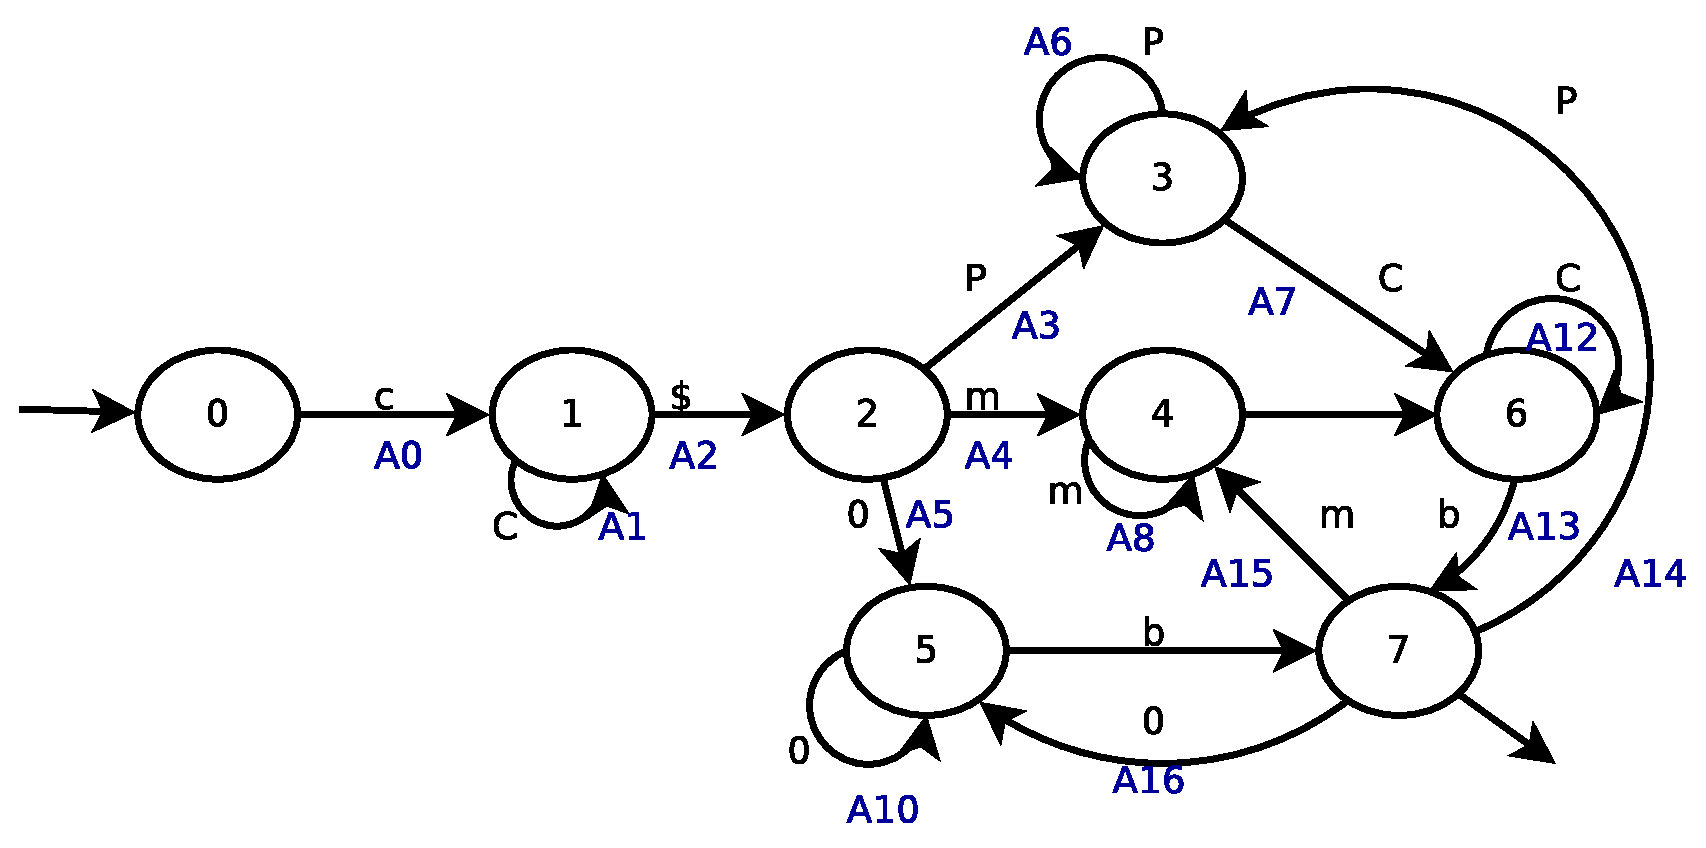
\includegraphics[width=15cm]{Diagramme1.eps}
	\caption{Automate fini}
	\centering
\end{figure}
\lstinputlisting[language=Algo]{1-1.algo}

\subsection{Langage ALGOL60}
\begin{remarque}
	Une écriture en grammaire est également une écriture en langages, ainsi : 
	\begin{displaymath}
		P = \left\{ \begin{array}{ccc}
			A &\rightarrow& \alpha_1\\
			A &\rightarrow& \alpha_2\\
			&\cdots&\\
			A &\rightarrow& \alpha_n\\
		\end{array}\right.
		\Leftrightarrow
		L(A) = \alpha_1 + \alpha_2 + \cdots + \alpha_n
	\end{displaymath}
\end{remarque}
\subsubsection{Définition de la grammaire}
\begin{eqnarray*}
X &=&   \{0, \cdots, 9, +, -, ., e\}\\
N &=& \{I,J,K,L,M,N,O\}\\
S &=& O\\
P &=&I + \lambda = cP + \lambda
\end{eqnarray*}
\subsubsection{Système d'équation de langage égaux à G}
\begin{displaymath}
	\left\{
	\begin{array}{ccc}
	I &=& c + cI\\
	J &=& I +sI\\
	K &=& . I\\
	L &=& \underbrace{I + K + IK}_{Problème de régularité ?}\\
	M &=&  eJ\\
	N &=& \L + M + LM\\
	O &=&  N + sN
\end{array}\right.
\end{displaymath}

\begin{description}
	\item[I] Entier signé
	\item[c] $c \in \{0\cdots9\}$
	\item[J] Entier
	\item[s] $s \in \{+,-\}$
	\item[K] Partie fractionnaire
	\item[L] Nombre décimal
	\item[M] Partie exponentiel
	\item[N] Nombre non signé
	\item[O] Nombre
\end{description}

\begin{remarque}
	Un automate fini ne peut reconnaître que les langages réguliers, qui sont engendrés par des grammaires linéaires à droite.

	L'union de langages régulier engendre un langage régulier, de même le produit de deux langages réguliers donnent un langage régulier. 
\end{remarque}

Dans notre cas, $L$ ne pose donc aucun problème de régularité étant donné que $I$ et $K$ sont des langages réguliers ainsi, l'union et le produit de
langages réguliers engendrant des langages réguliers, $L$ sera régulier. 

Le problème pourrait se poser pour $L$ mais aussi pour $N$ et $M$ : la
réponse étant la même.

$O$ est régulier, on peut donc trouver un automate finis le reconnaissant.

\begin{eqnarray*}
	I &=&  c(\lambda + I)  cP\\
	P &=& I + \lambda = cP+\lambda\\
	J &=&  I+sI = cP+sI\\
	K &=& . I\\
	L &=& I+K+IK = \underline{c}P+.I + \underline{c}PK = \underbrace{c(P+PK)}_{Q} + .I\\ &=&  cQ+.I\\
	Q &=& P + PK = cP + \lambda + (cP+\lambda)K = cP + \lambda + cPK + K = c(\underbrace{P+PK}_{Q}) + .I + \lambda\\ &=&  cQ+.I+\lambda\\
	M &=& eJ\\
	N &=&  L+M+LM = cQ + .I + eJ + (cQ+.I)M = cQ + .I + eJ + cQM + .IM + .IM\\ &=& c(\underbrace{Q + QM}_{R}) + .(\underbrace{I+IM}_{S})+ eJ\\
	R &=& Q + QM = cQ+.I+\lambda+cQM+.IM+eJM = c(Q+QM) + .(I+IM)+ eJ+ \lambda\\
	S &=& I + IM = cP + cPM = c(P+PM)\\
	T &=& P+PM = cP+\lambda + cPM + \underbrace{eJ}^{M} = c(P+PM) = e + \lambda\\
	O &=& N + sN = cR+.S+eJJ+sN
\end{eqnarray*}

D'où le système d'équation de langage suivant : 
\begin{displaymath}
	\left\{ \begin{array}{ccc}
		I &=& cP\\
		P &=&cP+\lambda\\
		J &=& cP+sI\\
		K &=&  .I\\
		L &=& cQ+.I\\
		Q &=&  cQ+.I+\lambda\\
		M &=& eJ\\
		N &=&  cR+.S+eJ\\
		R &=& cR + .s+eJ+\lambda\\
		S &=& cT\\
		T &=& cT+eJ+\lambda\\
		O &=&  cR+.s+eJ+sN\\
	\end{array}
	\right.
\end{displaymath}

L'axiome $O$ est un état initial et \{T,R,Q,P\} sont des états finaux.

\begin{figure}[H]
	\centering
	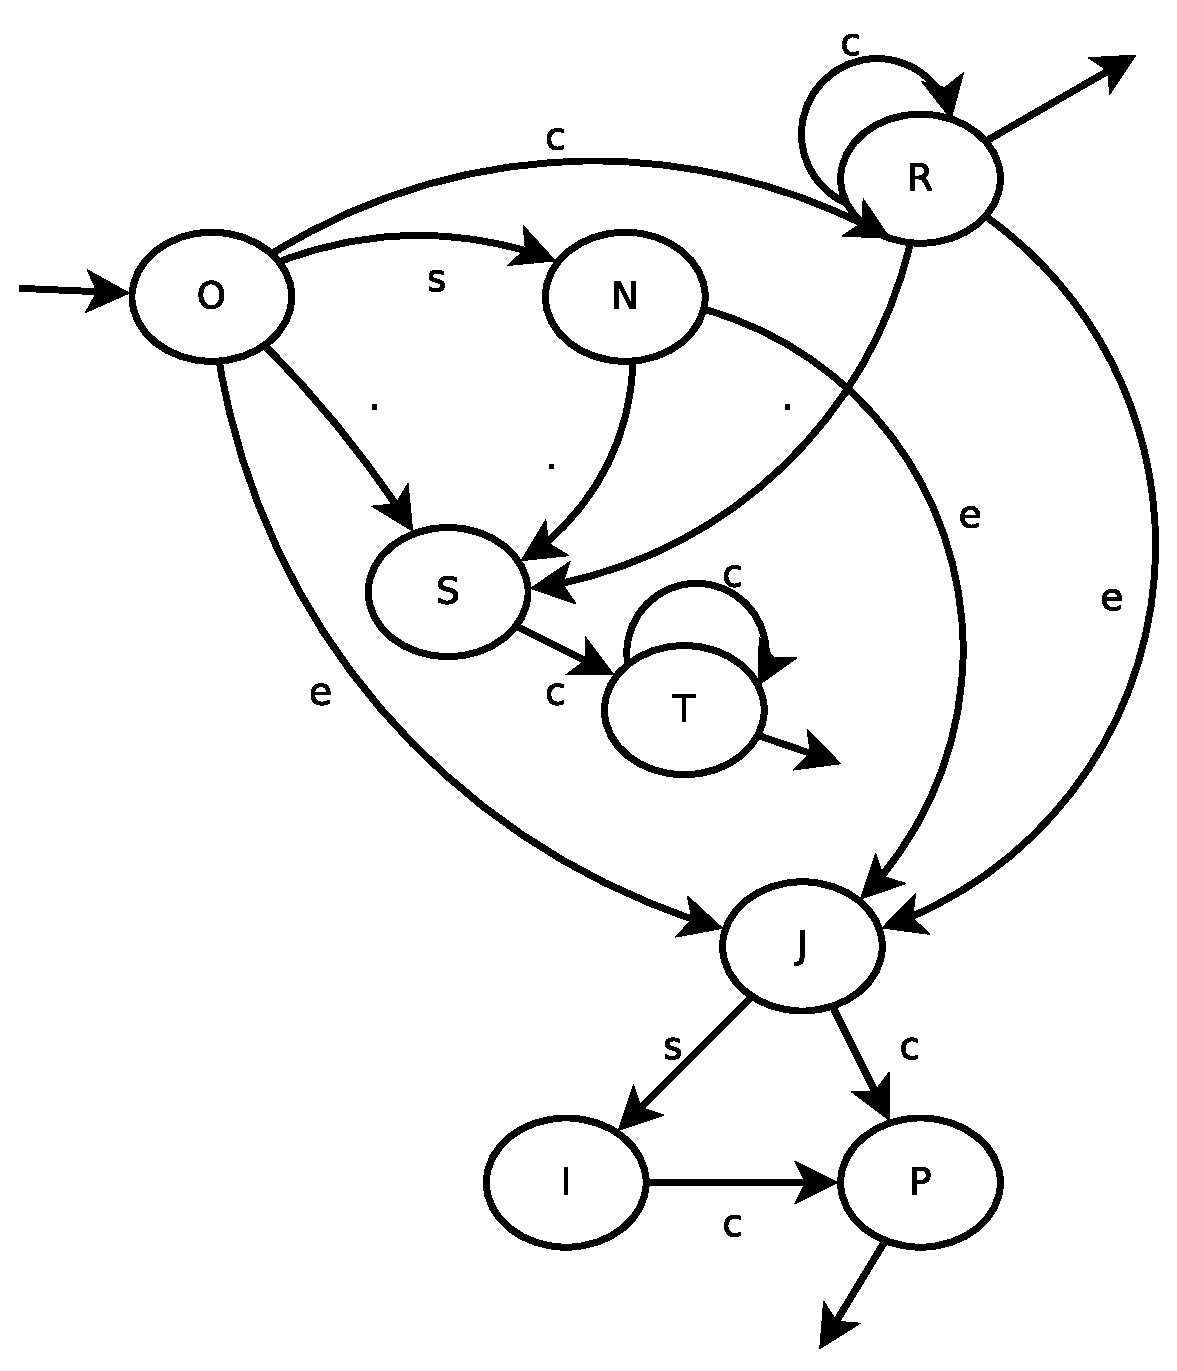
\includegraphics[width=12cm]{Diagramme2.eps}
	\caption{Automate fini}
\end{figure}

\section{Systèmes d'équations algébriques de langages}
\begin{remarque}
	3 théorèmes :
	\begin{description}
		\item[Arden] $X = r_1X + r_2 \Rightarrow X = r_1^*r_2$
		\item[Arden Bis] $X = Xr_{1}+r_2 \Rightarrow X = r_2r_1^*$
		\item[AnBn] $X = Yr_1+r_ \Rightarrow X = r_2r_1^*$
	\end{description}
\end{remarque}

\subsection{G1}
\begin{eqnarray*}
	S &=&  S\underbrace{a}_{r_1} + \underbrace{b}_{r_2} \Rightarrow S\\
	&\stackrel{Ardenbis}{=}&  ba* = ba^n n\geq 0
\end{eqnarray*}

\subsection{G2}
\begin{displaymath}
	\left\{
	\begin{array}{ccc}
		S &=&  aSb + T \stackrel{AnBn}{\Longrightarrow} S = a^nTb^n, n \geq 0 = a^nb^+b^n n\geq 0\\
		T &=& Tb+b \stackrel{Ardenbis}{\Longrightarrow} \\
	\end{array}
	\right.
\end{displaymath}

\chapter{Gramaires LL(1) -- Descente récursive}
\section{}
\subsection{Firsts}
\begin{eqnarray}
	S' &\rightarrow& S\$\\
	S  &\rightarrow& bRS\\
	S  &\rightarrow& RcSa\\
	S  &\rightarrow& \lambda\\
	R  &\rightarrow& acR\\
	R  &\rightarrow& b\\
\end{eqnarray}

\begin{eqnarray*}
	first_1(R) &=&\{a,b\}\\
	first_1(S &=&  \{a,b,\lambda\}\\
	first_2(R) &=& \{ac,b\}\\
	first_2(S) &=& \{\underbrace{\lambda}_{2.3},\underbrace{bb}_{2.2 + R}\}
\end{eqnarray*}
\begin{remarque}
	Pour le $first_2(R)$, $ac$ est le préfixe de longueur 2 des mots prouits par R, et $b$ est le mot de longueur inférieur ou égale à 2 produit par
	R.
\end{remarque}

Nous avons chercher les $first$ intuitivement, cependant nous nous sommes servis de la formule suivante : $first_k(\alpha_1 \alpha_2 \cdots \alpha_n) =
first_k(first_k(\alpha_a)first(\alpha_2) \cdots first_k(\alpha_n)$

\subsection{Follows}
\begin{remarque}
	$follow_k(y) = \cup first_k(S follow_k(x)))$
\end{remarque}

%%%%% TODO
\paragraph{k = 2}
Pour s:
\begin{enumerate}
	\item $2lookahead(S \rightarrow bRS) first_2 (bRS follow_2(S)) = b first_1(RS follow_2(S)) = \{ba,bb\} = E_1)$
	\item $2lookahead(S \rightarrow RcSa) = first_2(Sa = follow_2(S)) = \{ac,bc\}$
	\item $2lookahead(S \rightarrow RcSa) = first_2(RcSa = follow_2(S)) = first_2(first_2(R)c\cdots) = \{ac,bc\}$
\end{enumerate}
\section{}
Grammaire d'axiome $\theta$ puis augmentée : 
\begin{displaymath}
	\left \{\begin{array}{ccc}
	S' &\rightarrow& \theta\$^R	\\
	\theta &\rightarrow& cR\;|.S\;|eJ\;|\;sN\\
	R &\rightarrow& cR \;|\; .S \;|\; J \;|\; \lambda\\
	S &\rightarrow& cT\\
	J &\rightarrow& cP\;|\;sI\\
	N &\rightarrow& cR\;|\;.S\;|\;eJ\\
	T &\rightarrow& cT\;|\;eJ\;|\;\lambda\\
	P &\rightarrow& cP\; |\;\lambda\\
	I &\rightarrow& cP
\end{array} \right .
\end{displaymath}
\subsection{LL(1) ?}
\begin{eqnarray*}
	1lookahead(\theta \rightarrow cR) &=& \{c\} = \{0,1,\cdots,9\}\\
	1lookahead(\theta \rightarrow .S) &=& \{.\}\\ 
	1lookahead(\theta \rightarrow eJ) &=& \{e\}\\ 
	1lookahead(\theta \rightarrow sN) &=& \{s\} = \{+,\; -\}
\end{eqnarray*}

\subsection{Vérifions pour R, T et P}
\subsubsection{$R$ ?}
\begin{eqnarray*}
	1lookahead(R \rightarrow \lambda) &=& first_1(\lambda.follow_1(R)) = \{\$\}\\ 
	1lookahead(R \rightarrow cR) &=& \{c\}\\
	1lookahead(R \rightarrow .S) &=& \{.\}\\
	1lookahead(R \rightarrow eJ) &=& \{e\}
\end{eqnarray*}
OK, pas de conflit

\subsubsection{$P$ ?}
$$follow_2(P) = \{\$\}$$
Ok, pas de conflit.

\subsubsection{$T$ ?}
\begin{eqnarray*}
	1lookahead(T \rightarrow \lambda) &=& first_1(\lambda follow_1(T)) = \{\$\}\\
	&\Rightarrow& follow_1(T) = follow_1(S) = follow_1(\theta) \cup follow_1(R) \cup follow_1(N) = \{\$\}
\end{eqnarray*}
Ok, pas de conflit

\begin{remarque}
	Si on a une grammaire linéaire à droite, on est sûr qu'elle est $LL(1)$.\\
	
	Quelque soit la règle de l'ensemble des règles de production P, $\forall A : A \rightarrow \lambda, A \rightarrow xB$
\end{remarque}

\subsection{Procédures de descente récursive}
A chaque $A\in N$ on associe une procédure de nom $A$ qui contient << l'image de $\beta$ >>.

\begin{displaymath}
	Si\ A \rightarrow \beta\ avec\ \left\{
	\begin{array}{ccccc}
		\beta &=& x\in X &\Longrightarrow& SKIP('x')\\
		\beta &=& \lambda &\Longrightarrow& NULL\\
		\beta &=& B \in N &\Longrightarrow& B\\
		\beta_1 &=&  \beta_1\beta_2 \cdots \beta_n &\Longrightarrow& image(\beta_1) ; image(\beta_2); \cdots; image(\beta_n);
	\end{array}
	\right .
\end{displaymath}
\\

\begin{displaymath}
	\left .
	\begin{array}{ccc}
	Si\ A &\rightarrow& \beta_1\\
	Si\ A &\rightarrow& \beta_1\\
	Si\ A &\rightarrow& \beta_1
\end{array}
\right\}
\Longleftrightarrow
\left .
\begin{array}{ccccc}
	&& 1lookahead(A \rightarrow \beta_1) &:& image\beta_1\\
	&|&\;1lookahead(A \rightarrow \beta_2) &:&image\beta_2\\
	&&&\vdots&\\
	&|&\;1lookahead(A \rightarrow \beta_n) &:&image\beta_n\\
	&|&\;Others &:& ERREUR;
\end{array}
\right .
\end{displaymath}

\begin{tabular}{ll}
\lstinputlisting[language=Algo]{1.algo}
&
\lstinputlisting[language=Algo]{2.algo}\\
&\\
\lstinputlisting[language=Algo]{3.algo}&
\lstinputlisting[language=Algo]{4.algo}
\end{tabular}

\section{}
\begin{eqnarray*}
	<program> &\rightarrow& program<suiteDct> begin <switchInst> end \\
	<suiteInst> &\rightarrow& <inst> | <suiteInst> ; <inst>\\
	<inst> &\rightarrow& if <exp> then <suiteInst> else <suiteInst> end if\\
	&& |while<exp> loop <suiteInst> endloop\\
	&& | repeat<suiteInst> until <exp> endloop \\
	<suiteDcl> &\rightarrow& \cdots\\
	<exp> &\rightarrow& \cdots
\end{eqnarray*}

\begin{remarque}
	\begin{itemize}
		\item Non terminal : $< \cdots >$
		\item Terminal : $X = \{program, begin, end, if, \cdots\}$
	\end{itemize}
\end{remarque}

\subsection{Procédure de descente récursive}
\subsubsection{LL(1) ?}
Pour $<program>$ : ok\\
Pour $<inst>$  : ok 
\begin{eqnarray*}
	1lookahead() &=& \{if\}\\
	1lookahead() &=& \{while\}\\
	1lookahead() &=& \{repeat\}
\end{eqnarray*}

Pour $<suiteInst>$ : 
\begin{eqnarray*}
	1look(<suiteInst> &\rightarrow& <inst>) = \{if, while, repeat\}\\
	1look(<suiteInst> &\rightarrow& <suiteInst> ; <inst>) = \{if, while, repeat\}\\
\end{eqnarray*}
La grammaire est non LL(1) car elle est récursive à gauche !, à cause de $<suiteInst> \rightarrow <suiteInst> ; <inst>$

On peut la transformer en une grammaire linéaire à droite grâce à Arden.

\begin{eqnarray*}
	A &\rightarrow& A\beta|\alpha \overbrace{\Longrightarrow}^{ArgenBis} = \alpha\beta^*
\end{eqnarray*}
Éliminer la récursivité à gauche : 
\begin{eqnarray*}
	L(A) &=&  \alpha\beta^* = \alpha L(A')\\
	L(A') &=& \beta^* \lambda \Longrightarrow \beta L(A') + \lambda
\end{eqnarray*}

Donc $<suiteInst> \rightarrow <inst> | <suiteInst> ; <inst>$ devient:
\begin{eqnarray*}
\overbrace{<suiteInst>}^A &\rightarrow& \overbrace{<inst>}^{\alpha}\overbrace{<suiteInstPrime>}^{A'}\\
<suiteInstPrime> &\rightarrow& ; <inst><suiteInstPrime>|\lambda
\end{eqnarray*}

On vérifie de nouveau qu'elle soit bien LL(1);

Pour <suiteInst> pas de problème, car une seule règle.

Pour $<suiteInstPrime>$:
\begin{eqnarray*}
1lookahead(<suiteInstPrime> \rightarrow ; <inst> \leftrightarrow) &=& \{;\}\\
1lookahead(<suiteInstPrime> \rightarrow \lambda) &=&  first_1(\lambda.follow_1(<suiteInstPrime>) \\&=&  \{end, endif, else, endloop, until\} = E_2.
\end{eqnarray*}

Donc $G'$ est LL(1).

\begin{tabular}{ll}
\lstinputlisting[language=Algo]{5.algo}
&
\lstinputlisting[language=Algo]{6.algo}
\end{tabular}

\paragraph{k = 2}
Pour s:
\begin{enumerate}
	\item $2lookahead(S \rightarrow bRS) first_2 (bRS follow_2(S)) = b first_1(RS follow_2(S)) = \{ba,bb\} = E_1$
	\item $2lookahead(S \rightarrow RcSa) = first_2(Sa = follow_2(S)) = \{ac,bc\}$
	\item $2lookahead(S \rightarrow RcSa) = first_2(RcSa = follow_2(S)) = first_2(first_2(R)c\cdots) = \{ac,bc\}$
\end{enumerate}
\chapter{Génération de code en quadruplets}
Mettre en œuvre un processus de traduction en quadruplets des structures de contrôle <repeatstat>, <forstat> et <casestat> par la méthode de la
descente récursive.

\begin{remarque}
	\paragraph{Rappels}
	\begin{lstlisting}
<statlist > := <inst> <suite>
<suite> := ; <statlist >  $\lambda$ 
<inst> := \ldots<ifstat><whilestat><repeatstat><forstat><casestat>\ldots
\end{lstlisting}
\paragraph{Méthodologie}
\begin{enumerate}
	\item Donner le schéma équivalent en quadruplets
	\item Inventaire des << problèmes >> et solution apportées
	\item Mise en œuvre des porcédures de descente récursive pour engendrer le schéma en quadruplets voulus en tenant compte des solutions
\end{enumerate}

\begin{enumerate}
	\item \texttt{<repeatstat> \dots=     repeat <statlist> until <exp> endrepeat}
	\item \texttt{<forstat> \dots=     for ident := <exp1> step <exp2> until <exp3>
		do <statlist> endfor }
	\item \texttt{<casestat> \dots=     case <exp> of <alternative> \{ ; <alternative> \}*
		otherwise <statlist> endcase
		}
	\item \texttt{<alternative> \dots= nombre : <statlist>}
\end{enumerate}
\end{remarque}
\section{}
\lstinputlisting[language=Algo]{7.algo}
\begin{figure}[H]
	\centering
\includegraphics[width=14cm]{repeatstat.eps}
\end{figure}
\end{document}
